\باب{ ثنائی نظام}

\حصہ{اعشاری نظامِ گنتی}

روز مرہ زندگی میں اعشاری نظامِ گنتی استعمال ہوتا ہے، جو \عددی{0} تا \عددی{9} کے ہندسوں پر مبنی ہے۔کسی بھی گنتی کے نظام میں کل علامات کی تعداد کو اس نظام کی اساس کہتے ہیں۔اعشاری نظام میں \عددی{0} تا \عددی{9}، یعنی دس \عددی{10} علامات ہیں، یوں اعشاری نظام کی اساس دس ہے اور اس کو اساس \عددی{10} کا نظام کہتے ہیں۔

	مساوات \حوالہ{مساوات_ثنائی_عدد} میں \عددی{538.72} کو اعشاری نظام میں لکھتے ہوئے زیر نوشت میں \عددی{10} لکھا گیا ہے، جو اس بات کی یاد دہانی کراتا ہے کہ یہ عدد اساس دس کے نظام میں لکھا گیا ہے۔اس کتاب میں چونکہ کئی نظامِ گنتی استعمال ہوں گے، لہٰذا جہاں متن سے واضح نہ ہو وہاں اعداد کے ساتھ ان کی اساس زیر نوشت میں لکھی جائے گا۔
\begin{align}\label{مساوات_ثنائی_عدد}
538.72_{10}
\end{align}
اس نظام میں اعشاریہ کی بائیں جانب پہلا ہندسہ اکائی وزن رکھتا ہے، دوسرا دہائی، تیسرا سینکڑا، وغیرہ۔یوں مساوات \حوالہ{مساوات_ثنائی_سینکڑا} میں دیے گئے ہندسوں میں \عددی{8} کا 
مطلب \عددی{8\times 10^0=8\times 1=8_{10}} ہے، جبکہ \عددی{3} کا مطلب \عددی{3\times 10^1=30_{10}} اور \عددی{5} کا \عددی{5\times 10^2=500_{10}} ہے۔اسی طرح اعشاریہ کے دائیں جانب پہلے ہندسے کا وزن ایک بٹا دس ہے، دوسرے ہندسے کا ایک بٹا سو، اور تیسرے ہندسے کا ایک بٹا ہزار، وغیرہ۔یوں اس عدد میں \عددی{7} دراصل \عددی{7\times 10^{-1}=0.7_{10}} جبکہ \عددی{2} دراصل \عددی{2\times 10^{-2}=0.02_{10}} ہے۔
\begin{align}\label{مساوات_ثنائی_سینکڑا}
538.72_{10}=(5\times 10^2)+(3\times 10^1)+(8\times 10^0)+(7\times 10^{-1})+(2\times 10^{-2})
\end{align}

اس حقیقت کو درج ذیل عمومی روپ میں لکھ سکتے ہیں۔
\begin{multline}\label{مساوات_ثنائی_عمومی_روپ}
\cdots \,a_2\times 10^2+a_1\times 10^1+a_0\times 10^0+a_{-1}\times 10^{-1}+a_{-2}\times 10^{-2}\, \cdots\\
=(\cdots a_2a_1a_0\, .\, a_{-1}a_{-2}\cdots)_{10}
\end{multline}

 عدد \عددی{538.72_{10}} کو \عددی{x} لیتے ہوئے، شکل \حوالہ{شکل_ثنائی_ہندسوں_کے_نام} میں اس کے مختلف ہندسوں کو پکارنے کا طریقہ دکھایا گیا ہے، جس کے تحت \عددی{5} کو \عددی{x_2} جبکہ \عددی{3} کو \عددی{x_3} کہیں گے، وغیرہ۔

\begin{figure}
\centering
\begin{subfigure}{0.45\textwidth}
\centering
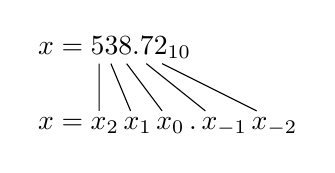
\begin{tikzpicture}
%\draw[step=1,thick](-4,-4) grid (4,1);
%\draw[step=0.1,gray](-4,-4) grid (4,1);
\draw (0,0)node[right]{$x=538.72_{10}$};
\draw(0,-1)node[right]{$x=x_2\, x_1\, x_0\, .\, x_{-1}\,x_{-2}$};
\draw(0.9,-0.2) --(0.9,-0.8) (1.05,-0.2)--(1.3,-0.8) (1.25,-0.2)--(1.7,-0.8) (1.5,-0.2)--(2.25,-0.8) (1.7,-0.2)--(2.9,-0.8);
\end{tikzpicture}
\end{subfigure}\hfill
\begin{subfigure}{0.45\textwidth}
\centering
\begin{tikzpicture}
\begin{tabular}{R}
x_2=5\\
x_1=3\\
x_0=8\\
x_{-1}=7\\
x_{-2}=2
\end{tabular}
\end{tikzpicture}
\end{subfigure}
\caption{عدد کے ہندسوں کو پکارنے کا طریقہ کار۔}
\label{شکل_ثنائی_ہندسوں_کے_نام}
\end{figure}

	اس طرح کسی بھی عدد میں بائیں جانب ہندسے کا رتبہ دائیں جانب ہندسے کے رتبہ سے بلند ہو گا۔مساوات \حوالہ{مساوات_ثنائی_عدد} میں بلند تر رتبے کا ہندسہ \عددی{5} ہے ، جبکہ کم تر رتبے کا ہندسہ \عددی{6 }ہے۔یوں \عددی{5} \اصطلاح{ بلند تر رتبی ہندسہ }\فرہنگ{بلند تر رتبی ہندسہ}\حاشیہب{most significant digit}\فرہنگ{most significant digit} جبکہ \عددی{6} \اصطلاح{ کم تر رتبی ہندسہ }\فرہنگ{کم تر رتبی ہندسہ}\حاشیہب{lowest significant digit}\فرہنگ{lowest significant digit} کہلاتے ہیں۔
	
	مساوات \حوالہ{مساوات_ثنائی_ہندسوں} میں سات کو تین مختلف طریقوں سے لکھا گیا ہے۔روز مرہ زندگی میں سات پہلی طرز پر لکھا جاتا ہے۔یوں کاغذ پر لکھتے ہوئے کسی بھی عدد کے بائیں جانب صفر نہیں لکھے جاتے اور عدد کے بائیں جانب کاغذ کو خالی چھوڑا جاتا ہے۔یہاں یہ بات سمجھنا ضروری ہے کہ روز مرہ زندگی میں اعداد لکھتے وقت ان کی لمبائی یا ان میں کُل ہندسوں کی تعداد پہلے سے متعین نہیں کی جاتی۔کمپیوٹر میں چیزیں کچھ مختلف ہیں، جہاں صرف صفر \عددی{0} اور ایک \عددی{1} کا وجود ممکن ہے۔کسی مقام پر اگر \عددی{1} نہیں لکھا ہو تو اس پر \عددی{0} لکھا ہو گا۔یوں کسی بھی عدد کے بائیں جانب خالی جگہ کا کمپیوٹر میں کوئی مطلب نہیں۔یہاں \عددی{0} یا \عددی{1} کا ہونا ضروری ہے۔کمپیوٹر میں ہر قسم کی معلومات لکھنے سے پہلے اس بات کا فیصلہ کیا جاتا ہے کہ اسے لکھنے کی خاطر کتنی جگہ درکار ہو گی۔یوں اگر عدد کو لکھنے کی خاطر تین ہندسوں کے لکھے جانے کے برابر جگہ مختص کی گئی ہو تو اس تمام جگہ کو ہر صورت استعمال کرنا ہوگا ، مثلاً سات کو \عددی{7} کی بجائے \عددی{007} لکھنا ہو گا۔
\begin{gather}
\begin{aligned}\label{مساوات_ثنائی_ہندسوں}
7_{10} &\\
07_{10}&\\
007_{10}&
\end{aligned}
\end{gather}

	اعشاری نظام میں گنتی \عددی{0_{10}} سے شروع ہوتی ہے اور بتدریج بڑھتے ہوئے \عددی{9_{10}} تک پہنچتی ہے۔ اس دوران دہائی، سینکڑا، وغیرہ کے مقام پر صفر رہتا ہے اور انہیں عام طور نہیں لکھا جاتا۔گنتی نو تک پہنچنے کے بعد دہائی، یعنی \عددی{10^1}، وزن رکھنے والے مقام پر \عددی{0} کی بجائے \عددی{1} لکھا جاتا ہے اور اکائی، یعنی \عددی{10^0}، وزن رکھنے والے مقام پر دوبارہ \عددی{0} تا \عددی{9} گنتی کی جاتی ہے۔ 
	
	اگر آپ کو اس پیراگراف کی سمجھ نہیں آئی تو اسے دوبارہ پڑھیں۔اس میں سادہ گنتی کی وضاحت کی گئی ہے۔ 
	
	اعشاری نظام میں اگر اعداد کو ایک ہندسے تک محدود کر دیا جائے تو اس میں \عددی{0_{10}} سے \عددی{9_{10}} تک گنتی ممکن ہو گی۔اگر اعداد کو دو ہندسوں تک محدود کر دیا جائے، یعنی اس میں زیادہ سے زیادہ دو ہندسے ہوں، تب \عددی{00_{10}} سے \عددی{99_{10}} تک گنتی ممکن ہو گی، اسی طرح تین ہندسوں تک کے عدد استعمال کرنے سے \عددی{000_{10}} سے \عددی{999_{10}} تک گنتی کی جا سکتی ہے، وغیرہ۔
	 


\حصہ{ہشتمی نظام گنتی}
	ہشتمی نظام \عددی{0} تا \عددی{7} ہندسوں پر مبنی ہے ۔اس نظام میں آٹھ ہندسے ہیں لہٰذا یہ اساس آٹھ نظام ہے۔بالکل اعشاری نظام کی طرح، اس نظام میں اعداد لکھتے ہوئے اعشاریہ کے بائیں جانب پہلے ہندسے کا وزن \عددی{8^0=1_{10}} ، دوسرے ہندسے کا \عددی{8^1=8_{10}} ، تیسرے کا \عددی{8^2=64_{10}}، وغیرہ، جبکہ اعشاریہ کے دائیں جانب پہلے ہندسے کا وزن \عددی{8^{-1}=0.125_{10}}، دوسرے کا \عددی{8^{-2}=0.015625_{10}} ہو گا، وغیرہ۔
\begin{gather}
\begin{aligned}\label{مساوات_ثنائی_آٹھ}
538.72_8&=[(5\times 8^2)+(3\times 8^1)+(8\times8^0)+(7\times 8^{-1})+(2\times 8^{-2})]_{10}\\
&=[(5\times 64)+(3\times 8)+(8\times 1)+(7\times 0.125)+(2\times 0.015625)]_{10}\\
&=[320+24+8+0.875+0.03125]_{10}\\
&=352.90625_{10}
\end{aligned}
\end{gather}

	 ہشتمی نظامِ گنتی کے لئے مساوات \حوالہ{مساوات_ثنائی_عمومی_روپ} درج ذیل روپ اختیار کرتی ہے۔
\begin{multline}
\cdots\, a_2\times 8^2+a_1\times 8^1+a_0\times 8^0+a_{-1}\times 8^{-1}+a_{-2}\times 8^{-2}\,\cdots\\
=(\cdots a_2a_1a_0\ . \,a_{-1}a_{-2}\cdots)_{8}
\end{multline}

	 ہشتمی نظام میں دیے گئے عدد کو اعشاری نظام میں تبدیل کرنا مساوات \حوالہ{مساوات_ثنائی_آٹھ} میں دکھایا گیا ہے۔ہشتمی عدد کے زیر نوشت میں \عددی{8} اس بات کی یاد دہانی کراتا ہے کہ یہ عدد ہشتمی نظام میں لکھا گیا ہے۔ 
	 
	اس نظام میں گنتی \عددی{0} سے شروع ہوتی ہے، \عددی{7} تک پہنچنے کے بعد \عددی{8^1} وزن رکھنے والے مقام پر \عددی{0} کی بجائے \عددی{1} لکھا جاتا ہے اور \عددی{8^0} وزن رکھنے والے مقام پر دوبارہ \عددی{0}سے \عددی{7} کی گنتی شروع ہوتی ہے۔

\حصہ{ثنائی نظامِ گنتی} 
	مائکروکنٹرولر کی دنیا میں ثنائی نظامِ گنتی استعمال ہوتا ہے۔ثنائی نظام دو ہندسوں، \عددی{0} اور \عددی{1}، پر مبنی ہے، لہٰذا یہ اساس دو کا نظام ہے۔
	اس نظام میں گنتی \عددی{0} سے شروع ہوتی ہے، \عددی{1} تک پہنچنے کے بعد \عددی{2^1} وزن رکھنے والی مقام پر \عددی{0} کی بجائے \عددی{1} لکھا جاتا ہے، اور \عددی{2^0} وزن رکھنے والے مقام پر دوبارہ \عددی{0} سے \عددی{1} گنتی شروع ہوتی ہے۔اس نظام میں گنتی کو مساوات \حوالہ{مساوات_ثنائی_گنتی} میں دکھایا گیا ہے، جہاں زیر نوشت میں اساس لکھنے سے گریز کیا گیا ہے۔موازنہ کے لئے اعشاری گنتی بھی پیش کی گئی ہے۔
\begin{gather}
\begin{aligned}\label{مساوات_ثنائی_گنتی}
0&=\phantom{000}0 &\quad \quad \quad &16=10000\\
1&=\phantom{000}1 &\quad \quad \quad &17=10001\\
2&=\phantom{00}10 &\quad \quad \quad &18=10010\\
3&=\phantom{00}11 &\quad \quad \quad &19=10011\\
4&=\phantom{0}100 &\quad \quad \quad &20=10100\\
5&=\phantom{0}101 &\quad \quad \quad &21=10101\\
6&=\phantom{0}110 &\quad \quad \quad &22=10110\\
7&=\phantom{0}111 &\quad \quad \quad &23=10111\\
8&=1000 &\quad \quad \quad &24=11000\\
9&=1001 &\quad \quad \quad &25=11001\\
10&=1010 &\quad \quad \quad &26=11010\\
11&=1011 &\quad \quad \quad &27=11011\\
12&=1100 &\quad \quad \quad &28=11100\\
13&=1101 &\quad \quad \quad &29=11101\\
14&=1110 &\quad \quad \quad &30=11110\\
15&=1111 &\quad \quad \quad &31=11111\\
\end{aligned}
\end{gather}
	اس نظام میں اعداد لکھتے ہوئے اعشاریہ کے بائیں جانب پہلے ہندسے کا وزن \عددی{2^0=1_{10}} ہو گا، دوسرے ہندسے کا \عددی{2^1=2_{10}} ، تیسرے کا \عددی{2^2=4_{10}}، وغیرہ، جبکہ اعشاریہ کے دائیں جانب پہلے ہندسے کا وزن \عددی{2^{-1}=0.5_{10}} ،دوسرے کا \عددی{2^{-2}=0.25_{10}} ہو گا۔
	
	 ثنائی نظامِ گنتی کے لئے ی مساوات \حوالہ{مساوات_ثنائی_عمومی_روپ} درج ذیل روپ اختیار کرتی ہے۔
\begin{multline}\label{مساوات_ثنائی_عمومی_روپ_ثنائی}
\cdots\, b_2\times 2^2+b_1\times 2^1+b_0\times 2^0+b_{-1}\times 2^{-1}+b_{-2}\times 2^{-2}\,\cdots\\
=(\cdots b_2b_1b_0\, .\, b_{-1}b_{-2}\cdots)_{2}
\end{multline}
	مساوات \حوالہ{مساوات_ثنائی_مثال} میں ثنائی نظام میں دیے گئے عدد کو اعشاری نظام میں تبدیل کرنا دکھایا گیا ہے۔ ثنائی عدد کے زیر نوشت میں \عددی{2} اس بات کی یاد دہانی کراتا ہے کہ یہ عدد ثنائی نظام میں لکھا گیا ہے۔
\begin{gather} 
\begin{aligned}\label{مساوات_ثنائی_مثال}
1011.1_2&=[(1\times 2^3)+(0\times 2^2)+(1\times 2^1)+(1\times 2^0)+(1\times 2^{-1})]_{10}\\
&=[(1\times 8)+(0\times 4)+(1\times 2)+(1\times 1)+(1\times 0.5)]_{10}\\
&=[8+0+2+1+0.5]_{10}\\
&=11.5_{10}
\end{aligned}
\end{gather}
	
 ثنائی عدد کے ہندسوں کو پکارنے کا طریقہ شکل \حوالہ{شکل_ثنائی_رتبہ_ہندسہ} میں دکھایا گیا ہے۔ ثنائی عدد کے دائیں ترین ہندسے کو  \اصطلاح{کم تر رتبی بِٹ }\فرہنگ{کم تر رتبی بِٹ}\حاشیہب{lowest significant it, LSB}\فرہنگ{LSB} یا  \اصطلاح{کم تر رتبی ثنائی ہندسہ}\فرہنگ{کم تر رتبی ثنائی ہندسہ}  یا بِٹ صفر یا بِٹ \عددی{b_0} کہیں گے؛ اس سے اگلے کو بِٹ ایک یا بِٹ \عددی{b_1} اور اس سے اگلے کو بِٹ دو یا بِٹ \عددی{b_2}، وغیرہ؛ جبکہ بائیں ترین ہندسے کو  \اصطلاح{بلند تر رتبی ثنائی ہندسہ }\فرہنگ{بلند تر رتبی ثنائی ہندسہ} یا  \اصطلاح{بلند تر رتبی بِٹ }\فرہنگ{بلند تر رتبی بِٹ}\حاشیہب{most significant bit, MSB}\فرہنگ{MSB}یا (موجودہ مثال میں) بِٹ سات یا بِٹ \عددی{b_7} کہیں گے۔

\begin{figure}
\centering
\begin{tikzpicture}
%\draw[step=1,thick](-4,-4) grid (4,1);
%\draw[step=0.1,gray](-4,-4) grid (4,1);
\draw (0,0)node[]{$10010101_2$};
\draw(-0.7,-0.2)--++(0,-0.2)--++(-0.5,-0.2)node[below left]{\text{\RL{\begin{minipage}{0.25\textwidth} 
بلند تر رتبی ثنائی ہندسہ\\
بلندتر رتبی بٹ\\
بِٹ سات\\
\عددی{b_7}
\end{minipage}}}};
\draw(0.55,-0.2)--++(0,-0.2)--++(0.5,-0.2)node[below right]{\text{\RL{\begin{minipage}{0.18\textwidth} 
کم تر رتبی ثنائی ہندسہ\\
کم تر رتبی بٹ\\
بِٹ صفر\\
\عددی{b_0}
\end{minipage}}}};
\end{tikzpicture}
\caption{بلند تر اور کم تر رتبی ہندسے۔}
\label{شکل_ثنائی_رتبہ_ہندسہ}
\end{figure}

اگر دیے گئے ثنائی عدد کے اعشاریہ کے دائیں جانب کچھ نہ ہو، تب درج ذیل لکھا جا سکتا ہے:
\begin{align}
1011_2=(2^3+2^1+2^0)_{10}=(8+2+1)_{10}=11_{10}
\end{align}
 جو ہندسے \عددی{1} ہیں، ان کے وزن جمع کیے جاتے ہیں۔

چار ہندسوں کا ثنائی عدد \عددی{0000_2} تا \عددی{1111_2} گنتی کر سکتا ہے؛ اس سے بڑا عدد لکھنے کے لئے چار سے زیادہ ہندسے درکار ہوں گے۔ مائکروکنٹرولر آٹھ ثنائی ہندسوں کے اعداد استعمال کرتا ہے جو \عددی{00000000_2} تا \عددی{11111111_2}، یعنی \عددی{0_{10}} تا \عددی{255_{10}} ظاہر کر سکتے ہیں۔

روز مرہ زندگی میں اعشاری نظامِ گنتی استعمال کرتے ہوئے اعداد لکھتے ہوئے ان کی بائیں جانب اضافی صفر نہیں لکھے جاتے، یعنی \عددی{27_{10}} کو \عددی{0027_{10}} نہیں لکھا جاتا۔کمپیوٹر کی دنیا میں اعداد عموماً آٹھ ہندسوں پر مبنی ثنائی عدد کی صورت میں لکھے جاتے ہیں؛ آٹھ سے کم ثنائی ہندسوں پر مبنی اعداد لکھتے ہوئے، بائیں جانب اضافی صفر لکھ کر انہیں آٹھ ہندسوں کی صورت دی جاتی ہے۔ یوں \عددی{27_{10}} کو ہم \عددی{101011_2} کی بجائے \عددی{00101011_2} لکھیں گے۔

\حصہ{اعشاری نظام سے ثنائی نظام میں تبادلہ}
اعشاری نظام میں دیے گئے عدد کو ثنائی نظام میں لکھنے کی خاطر اس عدد کو بار بار \عددی{2} سے تقسیم کریں، حتٰی کہ یہ مزید تقسیم نہ ہو سکے۔ہر مرتبہ تقسیم کے بعد حاصل باقی لیں؛ پہلے حاصل باقی کو ثنائی عدد کے سب سے کم وزن کے مقام پر لکھیں؛ اگلے حاصل باقی کو اس سے دگنے وزن کے مقام پر لکھیں؛ اسی طرح آخری حاصل باقی کو سب سے زیادہ وزن کے مقام پر لکھیں۔ یوں ثنائی عدد حاصل ہو گا۔	یہ طریقہ استعمال کرتے ہوئے \عددی{121_{10}} کو ثنائی لکھائی میں لکھتے ہیں۔

\عددی{121} کو \عددی{2} سے تقسیم کرنے سے حاصل تقسیم \عددی{60} اور باقی \عددی{1} ملتا ہے۔\\
\عددی{60} کو \عددی{2} سے تقسیم کرنے سے حاصل تقسیم \عددی{30} اور باقی \عددی{0} ملتا ہے۔\\
\عددی{30} کو \عددی{2} سے تقسیم کرنے سے حاصل تقسیم \عددی{15} اور باقی \عددی{0} ملتا ہے۔\\
\عددی{15} کو \عددی{2} سے تقسیم کرنے سے حاصل تقسیم \عددی{7} اور باقی \عددی{1} ملتا ہے۔\\
\عددی{7} کو \عددی{2} سے تقسیم کرنے سے حاصل تقسیم \عددی{3} اور باقی \عددی{1} ملتا ہے۔\\
\عددی{3} کو \عددی{2} سے تقسیم کرنے سے حاصل تقسیم \عددی{1} اور باقی \عددی{1} ملتا ہے۔\\
\عددی{1} کو \عددی{2} سے تقسیم کرنے سے حاصل تقسیم \عددی{0} اور باقی \عددی{1} ملتا ہے۔


اب سب سے آخری \قول{باقی} کو سب سے زیادہ وزن کے مقام پر اور سب سے پہلے \قول{باقی} کو سب سے کم وزن کے مقام پر لکھتے ہیں۔یوں \عددی{1111001_2} حاصل ہو گا، لہٰذا 
 \begin{align*}
 121_{10}=1111001_2
 \end{align*}
 ہو گا جہاں سات ثنائی ہندسے استعمال کیے گئے ہیں۔اپنی تسلی کے لئے اس عدد کو واپس اعشاری نظام میں منتقل کرتے ہیں۔
\begin{align*}
1111001_2=2^6+2^5+2^4+2^3+2^0=64+32+16+8+1=121_{10}
\end{align*}
اس طریقہ کار کی بہتر صورت پیش کرتے ہیں۔
\begin{otherlanguage}{english}
\begin{center}
\begin{tabular}{r|r|r}
2&121&\\
\hline
&60&1\\
\hline
&30&0\\
\hline
&15&0\\
\hline
&7&1\\
\hline
&3&1\\
\hline
&1&1\\
\hline
&0&1
\end{tabular}
\end{center}
\end{otherlanguage}
 عدد میں اعشاریہ کے بائیں جانب حصہ کو حصہ صحیح ، جبکہ دائیں حصہ کو حصہ مسکور یا کسری کہتے ہیں۔
\begin{align*}
\overbrace{xxxxxx}^{\text{\RL{حصہ صحیح}}} \, . \, \underbrace{yyyyyy}_{\text{\RL{حصہ مسکور}}}
\end{align*}
یوں \عددی{121.6875} میں \عددی{121} عدد صحیح اور \عددی{6875} عدد مسکور ہے۔

 عشری عدد کے صحیح حصہ کو ثنائی نظام میں تبدیل کرنا آپ سیکھ چکے؛ حصہ مسکور تبدیل کرنے کا طریقہ ذرہ مختلف ہے۔ آئیں یہ عمل سیکھیں۔
 
 
حصہ مسکور کو بار بار \عددی{2} سے ضرب دیں۔اگر حاصل ضرب کے اعشاریہ کے بائیں جانب \عددی{1} حاصل ہو تو اس کو حاصل ضرب سے ہٹا کر ثنائی عدد کے دائیں جانب منسلک کریں ورنہ ثنائی عدد کے دائیں جانب \عددی{0} منسلک کریں۔اس عمل کو ایک مثال کی مدد سے سیکھتے ہیں۔ 
\begin{otherlanguage}{english}
\begin{center}
\begin{tabular}{R|L}
\toprule
 &\text{\RL{ثنائی}}\\
\midrule
2\times 0.6875=1.375 & 0.1\\
2\times 0.3750=0.750&0.10\\
2\times 0.7500=1.500&0.101\\
2\times 0.5000=1.000&0.1011\\
\bottomrule
\end{tabular}
\end{center}
\end{otherlanguage}
یوں \عددی{0.6875_{10}=0.1011_2} ہو گا ؛ آخر میں دونوں حصوں کو ملا کر ثنائی عدد حاصل کرتے ہیں۔
\begin{align*}
121.6875_{10}=111001.1011_2
\end{align*}

\حصہ{اساس سولہ (سادس عشری) نظام گنتی}
	اساس سولہ کے نظام  ، جسے\اصطلاح{ سادس عشری }\فرہنگ{سادس عشری}\حاشیہب{hexadecimal}\فرہنگ{hexedecimal} نظام اور ششدہی نظام بھی کہتے ہیں، میں اعداد کی سولہ علامتیں ہیں۔ان میں پہلی دس علامتیں \عددی{0} تا \عددی{9} ہیں، جبکہ باقی علامتیں، بڑی لکھائی میں انگریزی حروف تہجی کے پہلے چھ  حروف یعنی \عددی{A}، \عددی{B}، \عددی{C}، \عددی{D}، \عددی{E} اور \عددی{F} ہیں۔ علامت \عددی{A} دس \عددی{(10_{10})} کو ظاہر کرتی ہے، یعنی \عددی{A=10_{10}} ہے ، جبکہ \عددی{B} گیارہ کو ، \عددی{B=11_{10}}، اور اسی طرح چلتے ہوئے \عددی{ F} پندرہ کو ظاہر کرتی ہے۔مساوات \حوالہ{مساوات_ثنائی_تمام} میں مختلف نظام دیے گئے ہیں۔ انہیں سمجھے بغیر آگے ہرگز مت بڑھیں۔ 
\begin{gather}
\begin{aligned}\label{مساوات_ثنائی_تمام}
&00_{10}=00_8=0000_2=0_{16}\\
&01_{10}=01_8=0001_2=1_{16}\\
&02_{10}=02_8=0010_2=2_{16}\\
&03_{10}=03_8=0011_2=3_{16}\\
&04_{10}=04_8=0100_2=4_{16}\\
&05_{10}=05_8=0101_2=5_{16}\\
&06_{10}=06_8=0110_2=6_{16}\\
&07_{10}=07_8=0111_2=7_{16}\\
&08_{10}=10_8=1000_2=8_{16}\\
&09_{10}=11_8=1001_2=9_{16}\\
&10_{10}=12_8=1010_2=A_{16}\\
&11_{10}=13_8=1011_2=B_{16}\\
&12_{10}=14_8=1100_2=C_{16}\\
&13_{10}=15_8=1101_2=D_{16}\\
&14_{10}=16_8=1110_2=E_{16}\\
&15_{10}=17_8=1111_2=F_{16}
\end{aligned}
\end{gather}
سادس عشری  نظام میں اشاریہ کی بائیں جانب پہلے ہندسے کا وزن \عددی{16^0=1_{10}}، دوسرے کا \عددی{16^1=16_{10}}، اور تیسرے کا \عددی{16^2=256_{10}} ہو گا۔ 

مساوات \حوالہ{مساوات_ثنائی_سادس} میں سادس عشری یا اساس سولہ نظام میں دیے گئے عدد کو اعشاری نظام میں تبدیل کرنا دکھایا گیا ہے۔ایسا کرتے ہوئے \عددی{A=10_{10}} اور \عددی{C=12_{10}} لئے گئے۔
\begin{gather}
\begin{aligned}\label{مساوات_ثنائی_سادس}
3AC.8_{16}&=(3\times 16^2)_{10}+(10\times 16^1)_{10}+(12\times 16^0)_{10}+(8\times 16^{-1})_{10}\\
&=(3\times 256)_{10}+(10\times 16)_{10}+(12\times 1)_{10}+(8\times 0.0625)_{10}\\
&=(768+160+12+0.5)_{10}\\
&=940.5_{10}
\end{aligned}
\end{gather}

	مساوات \حوالہ{مساوات_ثنائی_عمومی_روپ} اساس سولہ کے لئے درج ذیل ہو گی۔
\begin{multline}\label{مساوات_ثنائی_عمومی_روپ_سادس}
\cdots\,a_2\times 16^2+a_1\times 16^1+a_0\times 16^0+a_{-1}\times 16^{-1}+a_{-2}\times 16^{-2}\,\cdots\\
=(\cdots a_2a_1a_0\, .\, a_{-1}a_{-2}\cdots)_{16}
\end{multline}
 

\حصہ{اساس دو کا اساس آٹھ میں تبادلہ}
	مساوات \حوالہ{مساوات_ثنائی_تبدیلی_آٹھ} میں بائیں ہاتھ ثنائی عدد دیا گیا ہے۔ اعشاریہ سے شروع کرتے ہوئے، اعشاریہ کی دونوں جانب تین تین ہندسوں کے گروہ میں، اس ثنائی عدد کو لکھیں۔اعشاریہ کی بائیں جانب اگر آخر میں تین ہندسوں کا گروہ پورا نہ ہو تو بائیں اضافی صفر منسلک کر کے تین ہندسوں کا گروہ پورا کریں؛ اسی طرح اعشاریہ کی دائیں جانب اگر آخر میں تین ہندسوں کا گروہ پورا نہ ہو تو دائیں جانب اضافی صفر منسلک کر کے تین ہندسوں کا گروہ پورا کریں۔اب مساوات \حوالہ{مساوات_ثنائی_تمام} کی مدد سے ان تین تین کے گروہ کی جگہ ان کا مساوی اساس آٹھ ہندسہ لکھیں۔مساوات \حوالہ{مساوات_ثنائی_تبدیلی_آٹھ} میں یوں دو مقامات پر \عددی{100_2} کی جگہ \عددی{4_8} لکھا گیا،جبکہ \عددی{101_2} کی جگہ \عددی{5_8}، اور \عددی{001_2} کی جگہ \عددی{1_8} لکھا گیا ہے۔اس طرح اس عدد کو اساس آٹھ میں منتقل کیا گیا۔یاد رہے، اعشاریہ اپنی جگہ برقرار رکھتا ہے۔
	\begin{gather}
	\begin{aligned}\label{مساوات_ثنائی_تبدیلی_آٹھ}
	1101100.1_2&=(001\,\, 101 \,\,100 \,. \,100)_2\\
	&=(\phantom{0} 1\,\,\quad 5\,\,\quad 4\,\,\,\, . \quad 4)_8\\
	&=154.4_8
	\end{aligned}
	\end{gather}

	%?????KKKKK am here
\حصہ{اساس دو کا اساس سولہ میں تبادلہ}
	ثنائی عدد کو اساس سولہ میں لکھنے کی خاطر ثنائی عدد کو اعشاریہ سے شروع کرتے ہوئے اعشاریہ کی دونوں جانب چار چار ہندسوں کے گروہ میں لکھیں۔اگر اعشاریہ کی بائیں جانب آخر میں چار ہندسوں کا گروہ پورا نہ ہو تو عدد کی بائیں جانب اضافی صفر منسلک کر کے چار ہندسوں کا گروہ پورا کریں؛ اسی طرح اگر اعشاریہ کی دائیں جانب آخر میں چار ہندسوں کا گروہ پورا نہ ہوں تو دائیں جانب اضافی صفر منسلک کر کے گروہ پورا کریں۔اب مساوات \حوالہ{مساوات_ثنائی_تمام} کی مدد سے ان چار چار کے گروہ کی جگہ ان کی مساوی اساس سولہ کا ہندسہ لکھیں۔ یوں مساوات \حوالہ{مساوات_ثنائی_سولہ_تبدیل} میں \عددی{1000_2} کی جگہ \عددی{8_{16}} لکھ کر، \عددی{1100_2} کی جگہ \عددی{C_{16}}، اور \عددی{0110_2} کی جگہ \عددی{6_{16}} لکھ کر اساس سولہ میں مساوی عدد حاصل کیا گیا۔ یاد رہے کہ اعشاریہ اپنی جگہ برقرار رکھتا ہے۔
\begin{gather}
\begin{aligned}\label{مساوات_ثنائی_سولہ_تبدیل}
1101100.1_2&=(0110 \,\,1100\, . \, 1000)_2\\
&=(\phantom{0}\, 6\,\,\quad \,C\quad\, .\quad 8)_{16}\\
&=6C.8_{16}
\end{aligned}
\end{gather}
\حصہ{ اساس آٹھ اور اساس سولہ سے اساس دو میں تبادلہ}
	انہیں طریقوں کو الٹ استعمال کرتے ہوئے اساس آٹھ اور اساس سولہ کے اعداد با آسانی اساس دو میں لکھے جا سکتے ہیں۔مساوات \حوالہ{مساوات_ثنائی_آٹھ_تبدیل_اساس} میں اساس آٹھ:
 \begin{gather}
 \begin{aligned}\label{مساوات_ثنائی_آٹھ_تبدیل_اساس}
 372.5_8&=(3\quad\quad \,\, 7\quad\quad 2\quad . \quad 5)_8\\
 &=(011\quad 111 \quad 010\,\,. \,\,\, 101)_2\\
 &=011111010.101_2
 \end{aligned}
 \end{gather}
 اور مساوات \حوالہ{مساوات_ثنائی_سولہ_تبدیل_اساس} میں اساس سولہ کو ثنائی عدد کی صورت میں لکھنا دکھایا گیا ہے۔ 
\begin{gather}
 \begin{aligned}\label{مساوات_ثنائی_سولہ_تبدیل_اساس}
 9A2F.7_{16}&=(\quad 9 \quad \quad A\quad\quad \,\, 2\quad \quad \, F\quad \quad . \quad \quad 7)_{16}\\
 &=(1001\quad 1010\quad 0010\quad 1111\quad . \quad 0111)_2\\
 &=(1001101000101111.0111)_2
 \end{aligned}
 \end{gather}
ہم نے دیکھا کہ ثنائی عدد کے ہندسوں کو تین تین کے گروہ میں لکھنے سے اساس آٹھ اور چار چار کے گروہ میں لکھنے سے اساس سولہ عدد حاصل کیا جا سکتا ہے۔ آئیں درج بالا مساوات میں حاصل ثنائی عدد سے اساس آٹھ اور اساس سولہ اعداد حاصل کریں۔
 \begin{align*}
 1001101000101111.0111_2&=(001\quad 001\quad 101\quad 000\quad 101\quad 111\,\, . \,\,011\quad 100)_2\\
 &=(\,\,1\quad \quad 1\quad \quad 5\quad \quad 0 \quad \quad 5\quad \quad 7\quad .\quad 3\quad \quad 4)_8\\
 &=115057.34_8\\
 1001101000101111.0111_2&=(1001\quad 1010\quad 0010\quad 1111\,\, . \,\,0111)_2\\
 &=(\,\,\,9\quad \quad \quad A\quad \quad 2\quad \quad \,\,F \quad . \quad 7)_{16}\\
 &=9A2F.7_{16}
 \end{align*}
	مساوات \حوالہ{مساوات_ثنائی_آٹھ_تبدیل_اساس} اور مساوات \حوالہ{مساوات_ثنائی_سولہ_تبدیل_اساس} کی آخری لکیروں میں ثنائی اعداد کو دیکھتے ہوئے بہت جلد انسان اکتا جاتا ہے، البتہ، انہیں مساوات میں جہاں ثنائی اعداد گروہ کی صورت میں لکھے گئے ہیں، وہاں انہیں سمجھنا آسان ہے۔ یہی وجہ ہے کہ ثنائی اعداد بالخصوص اور دیگر اعداد بالعموم گروہی صورت میں لکھے جاتے ہیں۔
	
\begin{figure}
\centering
\begin{tikzpicture}
\draw(0,0)node[]{$\underbrace{b_7b_6b_5b_4}_{\text{\RL{بالا ریزہ}}}\,\underbrace{b_3b_2b_1b_0}_{\text{\RL{زیریں ریزہ}}}$};
\end{tikzpicture}
\caption{ایک بائٹ دو ریزوں پر مشتمل ہو گا۔}
\label{شکل_ثنائی_ریزہ}
\end{figure}

ایک ہندسے پر مبنی ثنائی عدد کو  \اصطلاح{ثنائی ہندسہ }\فرہنگ{ثنائی ہندسہ}یا  \اصطلاح{بِٹ }\فرہنگ{بِٹ}\حاشیہب{bit}\فرہنگ{bit} کہتے ہیں؛ آٹھ ثنائی ہندسوں، ، یعنی آٹھ بِٹ، کے گروہ کو  \اصطلاح{ہشتمی ثنائی عدد }\فرہنگ{ہشتمی ثنائی عدد}یا  \اصطلاح{بائٹ }\فرہنگ{بائٹ}\حاشیہب{byte}\فرہنگ{byte} کہتے ہیں۔بائٹ کو عموماً چار چار ثنائی  ہندسوں  کے گروہ میں لکھا جاتا ہے، جنہیں\اصطلاح{  ریزہ }\فرہنگ{ریزہ}\حاشیہب{nibble}\فرہنگ{nibble} کہتے ہیں۔  زیریں چار بِٹ کو \قول{ زیریں ریزہ } جبکہ  بالا چار بِٹ کو \قول{ بالا ریزہ } کہیں گے (شکل  \حوالہ{شکل_ثنائی_ریزہ} دیکھیں)۔ یوں مساوات \حوالہ{مساوات_ثنائی_سولہ_تبدیل_اساس} میں دو بائٹ ہیں۔اسی مساوات کو الٹ چلاتے ہوئے یہ واضح ہے کہ ہشتمی ثنائی عدد کو چار چار ثنائی اعداد کے گروہ میں لکھ کر انہیں جلد اساس سولہ (سادس عشری روپ)   میں لکھا جا سکتا ہے۔

\حصہء{سوالات}
%Q1.1
\ابتدا{سوال}
درج ذیل اعشاری اعداد کو ثنائی روپ میں لکھیں۔
\begin{multicols}{4}
\begin{enumerate}[a.]

\item

 \(33\)

\item

 \(64\)

\item

 \(128\) 

\item

 \(256\)

\item

 \(4096\)

\item

 \(0.375\)

\item

 \(5.625\) 

\item

 \(13.6875\)
\end{enumerate}
\end{multicols}
جواب: \عددی{100001}، \عددی{1000000}، \عددی{10000000}، \عددی{100000000}، \عددی{1000000000000}، \عددی{0.011}، \عددی{101.101}، \عددی{1101.1011}
\انتہا{سوال}
\ابتدا{سوال}
%Q1.2
درج ذیل ثنائی اعداد کو اعشاری روپ میں لکھیں۔
\begin{multicols}{4}
\begin{enumerate}[a.]

\item  
 
 \(10\)  

\item  
 
 \(101\) 

\item  
 
 \(1101\)  

\item  
 
 \(11011\)

\item  
 
 \(101101011\) 

\item  
 
 \(11001010011\)  
\end{enumerate}
\end{multicols}
جواب: \عددی{2}، \عددی{5}، \عددی{13}، \عددی{27}، \عددی{363}، \عددی{1619}
\انتہا{سوال}
\ابتدا{سوال}
%Q1.3
درج ذیل ثنائی اعداد کو اعشاری روپ میں لکھیں۔
\begin{multicols}{4}
\begin{enumerate}[a.]

\item  
 
 \(10.1\)  
\item  
 
 \(101.01\)

\item  
 
 \(0.001101\) 
\item  
 
 \(1011.01101\)

\item  
 
 \(100.001\) 
\item  
 
 \(1111.1111\)
\end{enumerate}
\end{multicols}
جواب: \عددی{2.5}،   \عددی{5.25}،   \عددی{0.203125}،   \عددی{11.40625}،   \عددی{4.125}،   \عددی{15.9375}
\انتہا{سوال}
\ابتدا{سوال}
%Q1.4
درج ذیل اعشاری اعداد کو اساس سولہ اور اساس آٹھ میں تبدیل کریں۔
\begin{multicols}{4}
\begin{enumerate}[a.]

\item 
 \(7\) 
\item 
 \(23\) 
\item 
 \(32\) 
\item 
 \(64\)  

\item 
 \(1024\) 
\item 
 \(2048\)
\end{enumerate}
\end{multicols}
جواب:  اساس سولہ \عددی{7}، \عددی{17}، \عددی{20}، \عددی{40}، \عددی{400}، \عددی{800}؛ اساس آٹھ   \عددی{7}، \عددی{27}، \عددی{40}، \عددی{100}، \عددی{2000}، \عددی{4000}
\انتہا{سوال}
\ابتدا{سوال}
%Q1.5
درج ذیل اساس سولہ اعداد کو اساس آٹھ اور ثنائی روپ میں لکھیں۔
\begin{multicols}{4}
\begin{enumerate}[a.]

\item 
 \(7\) 
\item 
 \(10\) 
\item 
 \(1A\) 
\item 
 \(2B3\) 

\item 
 \(A.BC\) 
\item 
 \(0.12\) 
\item 
 \(F0\) 
\item 
 \(FFFF\)
\end{enumerate}
\end{multicols} 
جواب:اساس سولہ   \عددی{7}، \عددی{20}، \عددی{32}، \عددی{1263}، \عددی{12.57}، \عددی{0.044}، \عددی{360}، \عددی{177777}؛ ثنائی  \عددی{111}، \عددی{10000}، \عددی{11010}، \عددی{1010110011}، \عددی{1010.101111}، \عددی{0.0001001}، \عددی{11110000}، \عددی{1111111111111111}
\انتہا{سوال}
%=======================

